\documentclass[tikz]{standalone}
\usepackage{pgfplots}
\pgfplotsset{compat=1.15}
\usepackage{mathrsfs}
\usetikzlibrary{arrows,calc}
\usepackage{tkz-euclide}

\pagestyle{empty}

\definecolor{AngleClr}{rgb}{0,0.39215686274509803,0}
\definecolor{ShapeClr}{rgb}{0.6,0.2,0}
\definecolor{BlueClr}{RGB}{5,81,163}

\begin{document}

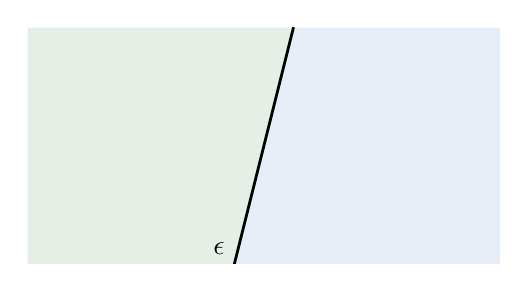
\begin{tikzpicture}[scale=.75]
\tkzSetUpLine[line width=1pt,color=black]
\tkzSetUpPoint[fill=black]

\tkzDefPoints{-2/0/A,2.5/0/B,1.5/-4/C,-2/-4/D,6/0/E,6/-4/F}

\clip (A) rectangle (F);

\tkzFillPolygon[fill=AngleClr,fill opacity=0.1](A,B,C,D)
\tkzFillPolygon[fill=BlueClr,fill opacity=0.1](B,E,F,C)
\tkzDrawSegments[line width=1pt](B,C)

\tkzLabelPoint[above left](C){$\epsilon$}

\end{tikzpicture}

\end{document}
